\section{Summary of Paper \ref{pap:ikeda}}
\subsection*{"\nameref{pap:ikeda}"}
\subsection*{Scope and motivations}
The impact of roll motions can be seen from the APL China casualty in 1998, where a post-Panamax C11 class container ship lost almost a third of its containers \cite{france_investigation_2001}. Another example is the container ship Svendborg Maersk, were 500 containers were lost overboard and 250 containers were damaged as a result of heavy roll motions during a passage from English Channel to Gibraltar \cite{danish_maritime_accident_investigation_board_marine_2014}.

Analyzing the ship's roll damping is therefore crucial, not the least in the earlier design stages of a ship, where efficient and accurate methods are needed. 
Getting the best possible accuracy with the lowest possible computational cost is an important factor. An explicit semi-empirical formula was proposed in Paper \ref{pap:rolldamping}, based on the simplified Ikeda's method \cite{kawahara_simple_2011}. This is an alternative with very low computational cost. However, it was also found to have poor accuracy, especially for modern ship designs. 

Paper \ref{pap:ikeda} proposed a new hybrid method, as a solution to this problem, where the viscous roll damping from Ikeda’s semi-empirical method was injected into an existing 3D unsteady fully nonlinear potential flow (FNPF) method \cite{kjellberg_fully_2013}.

\subsection*{Results and concluding remarks}
The viscous roll damping was calculated with Ikeda's method \cite{ikeda_components_1978} for the KVLCC2 test case. Error in the calculation of the $C_r$ coefficient to obtain the eddy damping at zero speed was encountered, which was found to originate from a regression formula from experiments conducted by \textcite{ikeda_eddy_1978} on a number of two-dimensional cylinders with various sections. A new regression was instead proposed, using a decision tree model.
Fig.\ref{fig:ikeda_sections} shows $C_r$ from the experiments and corresponding predictions with Ikeda's method and the decision tree. The capital letters refer to cylinder sections from the experiments
\cite{ikeda_eddy_1978}.
\begin{figure}[h]
\begin{center}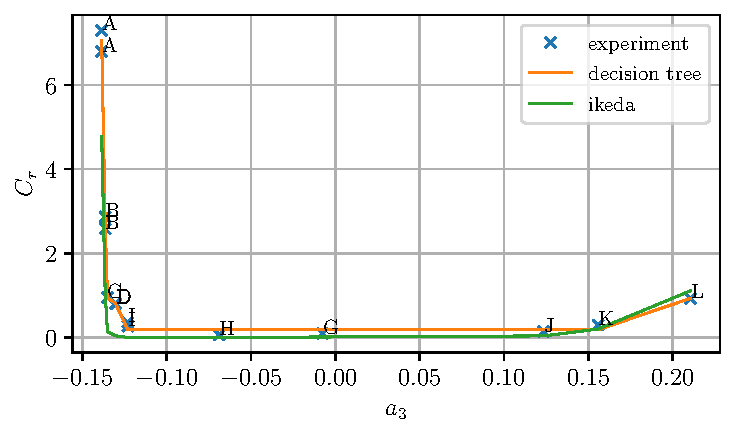
\includegraphics[\textwidth]{figures/ikeda_sections.pdf}\end{center}
\vspace{-0.4cm}
\caption{$C_r$ for cylinder sections from experiments and predicted with Ikeda's method and the decision tree model.}
\label{fig:ikeda_sections}
\end{figure}
\FloatBarrier

The total predicted roll damping was reasonably in good agreement with the damping of the model tests at zero speed (\autoref{fig:hybrid_0}) and very well in agreement at speed (\autoref{fig:hybrid_speed}).
\begin{figure}[h]
\begin{center}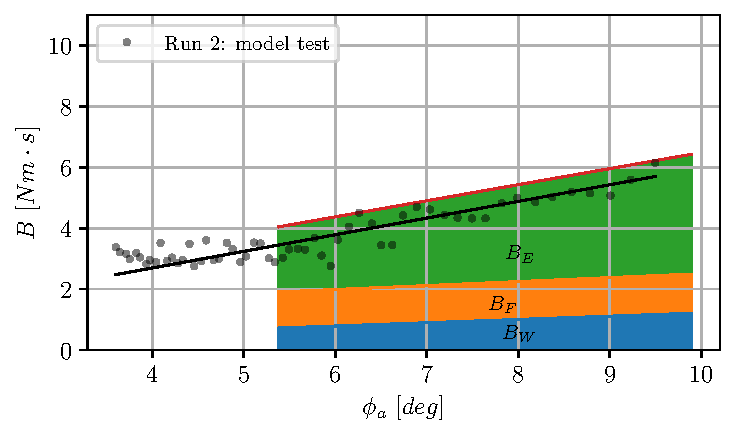
\includegraphics[\textwidth]{figures/hybrid_0.pdf}\end{center}
%\vspace{-0.4cm}
\caption{Roll damping from hybrid method ($F_n = 0$) for KVLCC2.}
\label{fig:hybrid_0}
\end{figure}
\begin{figure}[h]
\begin{center}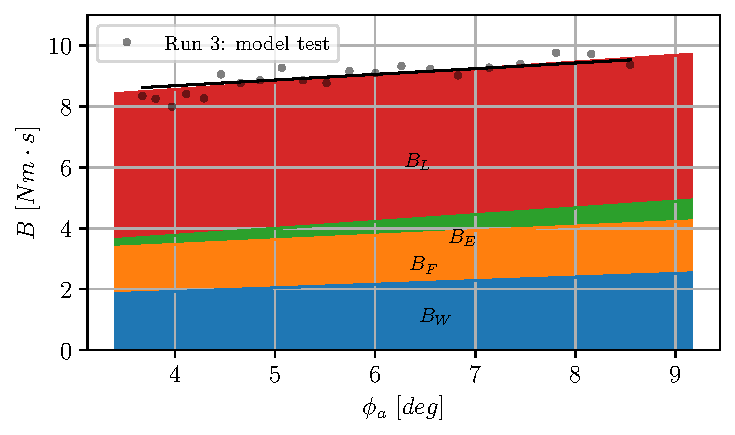
\includegraphics[\textwidth]{figures/hybrid_speed.pdf}\end{center}
%\vspace{-0.4cm}
\caption{Roll damping from hybrid method ($F_n = 0.14$) for KVLCC2.}
\label{fig:hybrid_speed}
\end{figure}
Roll decay simulations with damping from the hybrid method were conducted. Results from these simulations were compared with the model tests at zero speed (\autoref{fig:hybrid_0_time}) and at speed (\autoref{fig:hybrid_speed_time}). The time series from the corresponding FNPF
simulations have also been added to these plots to show how much the injection of semi-empirical viscous damping can improve the accuracy of these simulations.
\begin{figure}[h]
\begin{center}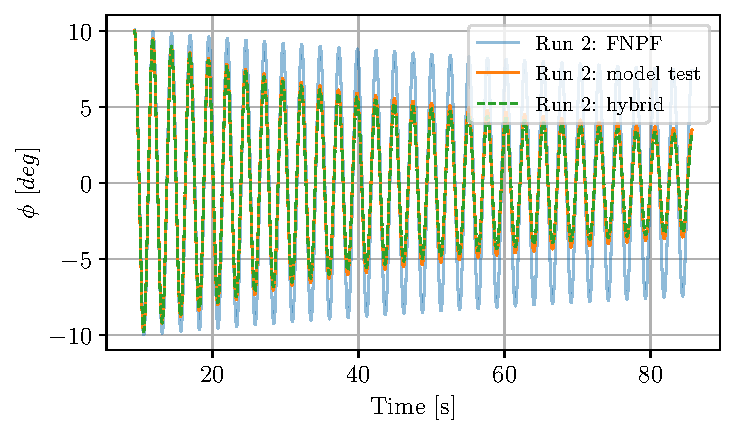
\includegraphics[\textwidth]{figures/hybrid_0_time.pdf}\end{center}
%\vspace{-0.7cm}
\caption{Roll decay ($F_n=0$) for KVLCC2.}
\label{fig:hybrid_0_time}
\end{figure}
\begin{figure}[h]
\begin{center}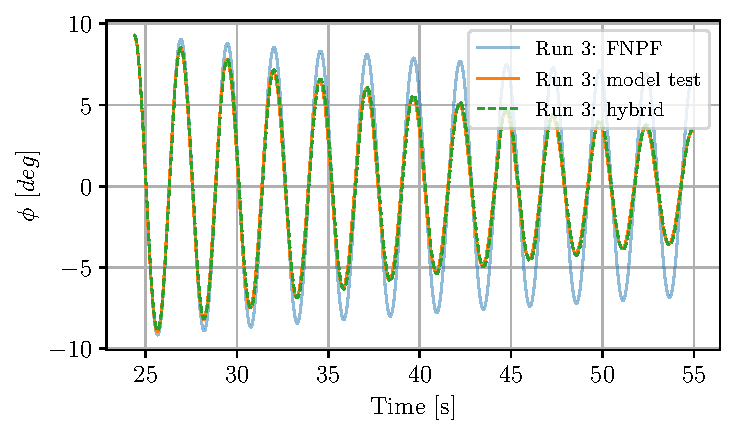
\includegraphics[\textwidth]{figures/hybrid_speed_time.pdf}\end{center}
%\vspace{-0.7cm}
\caption{Roll decay ($F_n=0.14$) for KVLCC2.}
\label{fig:hybrid_speed_time}
\end{figure}
\clearpage